\documentclass[a4paper, 11pt]{article}

\usepackage[czech]{babel}
\usepackage[utf8]{inputenc}
\usepackage[left=2cm, top=3cm, text={17cm, 24cm}]{geometry}
\usepackage{times}
\usepackage{multirow}
\usepackage[ruled, czech, linesnumbered, noline, longend]{algorithm2e}
\usepackage{graphics}
\usepackage{pdflscape}

\begin{document}

	\catcode`\-=12

	\begin{titlepage}
		\begin{center}
			\Huge
			\textsc{Vysoké učení technické v~Brně} \\
			\huge
			\textsc{Fakulta informačních technologií} \\
			\vspace{\stretch{0.382}}
			\LARGE
			Typografie a~publikování\,--\,3.~projekt \\
			\Huge
			Tabulky a~obrázky
			\vspace{\stretch{0.618}}
		\end{center}

		{\Large
			\today
			\hfill
			Elizaveta Syanova
		}
	\end{titlepage}


	\section{Úvodní strana}

	Název práce umístěte do zlatého řezu a~nezapomeňte uvést dnešní datum a~vaše jméno a~příjmení.


	\section{Tabulky}

	Pro sázení tabulek můžeme použít buď prostředí\texttt{ tabbing }nebo prostředí\texttt{ tabular}.


	\subsection{Prostředí\texttt{ tabbing}}

	Při použití\texttt{ tabbing }vypadá tabulka následovně:
	\begin{tabbing}
		Vodní melouny \quad	\= \textbf{Cena} \quad	\= \textbf{Množství}	\kill
		\textbf{Ovoce}		\> \textbf{Cena}		\> \textbf{Množství}	\\
		Jablka				\> 25,90				\> 3 kg					\\
		Hrušky				\> 27,40				\> 2,5 kg				\\
		Vodní melouny		\> 35,--				\> 1 kus				\\
	\end{tabbing}
	Toto prostředí se dá také použít pro sázení algoritmů, ovšem vhodnější je použít
	prostředí\texttt{ algorithm }nebo\texttt{ algorithm2e }(viz sekce~\ref{section:algoritmy}).


	\subsection{Prostředí\texttt{ tabular}}

	Další možností, jak vytvořit tabulku, je použít prostředí\texttt{ tabular}. Tabulky pak
	budou vypadat takto\footnotemark:
	\bigskip
	\begin{table}[h]
		\centering
		\begin{tabular}{| l | r | r |}
			\hline
							& \multicolumn{2}{c |}{\textbf{Cena}}	\\ \cline{2-3}
			\textbf{Měna}	& \textbf{nákup}	& \textbf{prodej}	\\ \hline
			EUR				& 25,277				& 26,943				\\
			GBP				& 29,368				& 31,492				\\
			USD				& 21,260				& 22,661				\\ \hline
		\end{tabular}
		\caption{Tabulka kurzů k~dnešnímu dni}
		\label{table:kurzy}
	\end{table}
	\bigskip
	\begin{table}[h]
		\centering
		\begin{tabular}[p]{| c | c |}
			\hline
			$ A $		& $ {\neg}A $	\\ \hline
			\textbf{P}	& N				\\ \hline
			\textbf{O}	& O				\\ \hline
			\textbf{X}	& X				\\ \hline
			\textbf{N}	& P				\\ \hline
		\end{tabular}
		\begin{tabular}[p]{| c | c | c | c | c | c |}
			\hline
			\multicolumn{2}{| c |}{\multirow{2}{*}{$ A \wedge B $}} & \multicolumn{4}{c |}{$ B $}
			\\ \cline{3-6}
			\multicolumn{2}{| c |}{} & \textbf{P} & \textbf{O} & \textbf{X}	& \textbf{N} \\ \hline
			\multirow{4}{*}{$ A $}	& \textbf{P} & P & O & X & N \\ \cline{2-6}
									& \textbf{O} & O & O & N & N \\ \cline{2-6}
									& \textbf{X} & X & N & X & N \\ \cline{2-6}
									& \textbf{N} & N & N & N & N \\ \hline
		\end{tabular}
		\begin{tabular}[p]{| c | c | c | c | c | c |}
			\hline
			\multicolumn{2}{| c |}{\multirow{2}{*}{$ A \vee B $}} & \multicolumn{4}{c |}{$ B $}
			\\ \cline{3-6}
			\multicolumn{2}{| c |}{} & \textbf{P} & \textbf{O} & \textbf{X}	& \textbf{N} \\ \hline
			\multirow{4}{*}{$ A $}	& \textbf{P} & P & P & P & P \\ \cline{2-6}
									& \textbf{O} & P & O & P & O \\ \cline{2-6}
									& \textbf{X} & P & P & X & X \\ \cline{2-6}
									& \textbf{N} & P & O & X & N \\ \hline
		\end{tabular}
		\begin{tabular}[p]{| c | c | c | c | c | c |}
			\hline
			\multicolumn{2}{| c |}{\multirow{2}{*}{$ A \rightarrow B $}} & \multicolumn{4}{c |}{$ B $}
			\\ \cline{3-6}
			\multicolumn{2}{| c |}{} & \textbf{P} & \textbf{O} & \textbf{X}	& \textbf{N} \\ \hline
			\multirow{4}{*}{$ A $}	& \textbf{P} & P & O & X & N \\ \cline{2-6}
									& \textbf{O} & P & O & P & O \\ \cline{2-6}
									& \textbf{X} & P & P & X & X \\ \cline{2-6}
									& \textbf{N} & P & P & P & P \\ \hline
		\end{tabular}
		\caption{
			Protože Kleeneho trojhodnotová logika už je \uv{zastaralá}, uvádíme si zde
			příklad čtyřhodnotové logiky
		}
		\label{table:logika}
	\end{table}
	\bigskip
	\footnotetext{
		Kdyby byl problem s\texttt{ cline,} zkuste se podívat třeba sem:
		http://www.abclinuxu.cz/tex/poradna/show/325037.
	}
	\pagebreak
	
	\label{section:algoritmy}
	
	\section{Algoritmy}

	Pokud budeme chtít vysázet algoritmus, můžeme použít prostředí\texttt{ algorithm\footnote{
		Pro nápovědu, jak zacházet s~prostředím\texttt{ algorithm,} můžeme zkusit tuhle stránku: \\
		http://ftp.cstug.cz/pub/tex/CTAN/macros/latex/contrib/algorithms/algorithms.pdf.
	} }
	nebo\texttt{ algorithm2e\footnote{
		Pro\texttt{ algorithm2e }zase tuhle:
		http://ftp.cstug.cz/pub/tex/CTAN/macros/latex/contrib/algorithm2e/doc/algorithm2e.pdf.
	}}. Příklad použití prostředí\texttt{ algorithm2e }viz Algoritmus~\ref{algorithm:fastslam}. \\
	\IncMargin{1.5em}
	\begin{algorithm}
		\caption{\textsc{FastSLAM}}
		\label{algorithm:fastslam}

		\SetNlSty{}{}{:}
		\SetNlSkip{0.4em}
		\SetAlgoNlRelativeSize{-1}
		\SetInd{1em}{1em}

		\Indm\Indmm
		\KwIn{$ (X_{t - 1}, u_t, z_t) $}
		\KwOut{$ X_t $}
		\Indp\Indpp
		\BlankLine

		$ \overline{X_t} = X_t = 0 $ \\

		\For{$ k = 1 \textrm{\emph{ to }} M $}{
			$ x_t^{[k]} = \emph{sample\_motion\_model}(u_t, x_{t - 1}^{[k]}) $ \\
			$ \omega_t^{[k]} = \emph{measurement\_model}(z_t, x_t^{[k]}, m_{t - 1}) $ \\
			$ m_t^{[k]} = updated\_occupancy\_grid(z_t, x_t^{[k]}, m_{t - 1}^{[k]}) $ \\
			$ \overline{X_t} = \overline{X_t} + \langle x_x^{[m]}, \omega_t^{[m]}  \rangle $ \\
		}

		\For{$ k = 1 \textrm{\emph{ to }} M $}{
			draw $ i $ with probability $ \approx \omega_t^{[i]} $ \\
			add $ \langle x_x^{[k]}, m_t^{[k]} \rangle \textrm{ to } X_t $ \\
		}

		\Return{$ X_t $}
	\end{algorithm}
	\DecMargin{1.5em}


	\section{Obrázky}

	Do našich článků můžeme samozřejmě vkládat obrázky. Pokud je obrázkem fotografie,
	můžeme klidně použít bitmapový soubor. Pokud by to ale mělo být nějaké schéma nebo
	něco podobného, je dobrým zvykem takovýto obrázek vytvořit vektorově.

	\begin{figure}[h]
		\centering
		\scalebox{0.4}{
			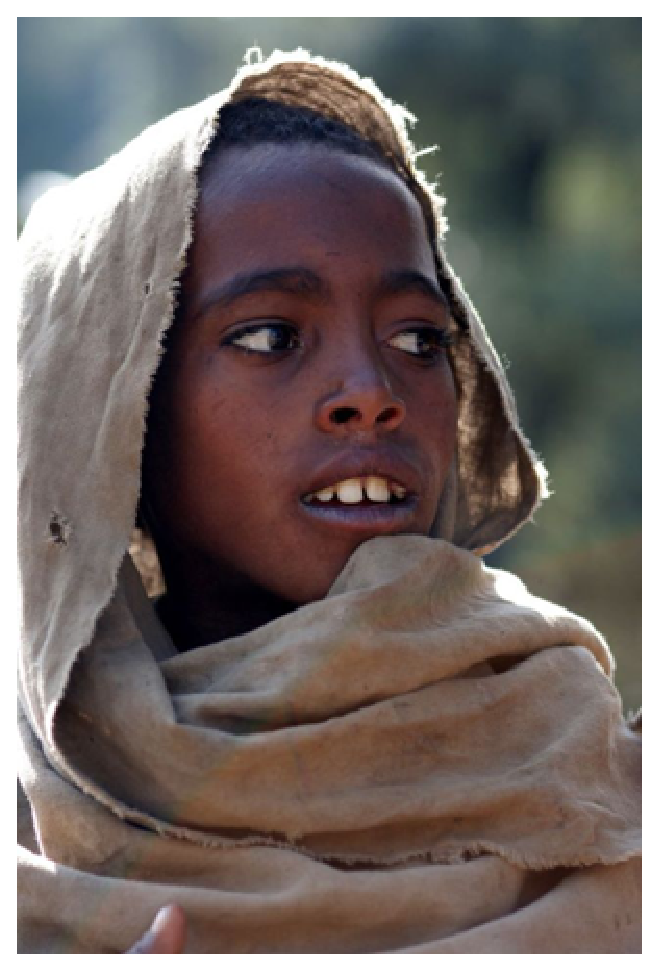
\includegraphics{etiopan.eps}
			\reflectbox{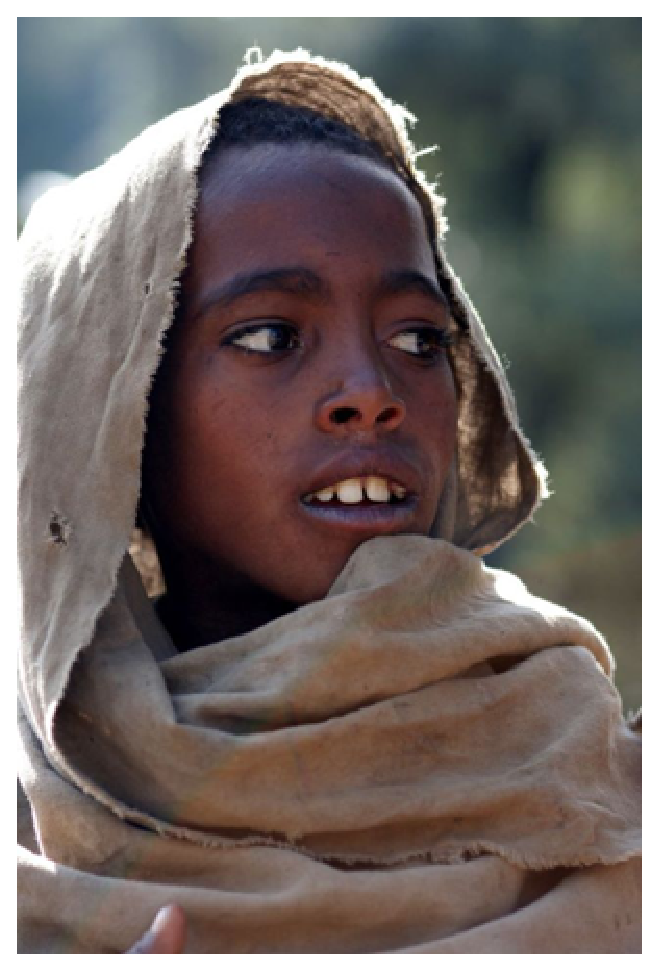
\includegraphics{etiopan.eps}}
		}
		\caption{Malý Etiopánek a~jeho bratříček}
		\label{figure:etiopan}
	\end{figure}
	\newpage

	Rozdíl mezi vektorovým\,\dots

	\begin{figure}[h]
		\scalebox{0.4}{
\includegraphics{oniisan.eps}}
		\centering
		\caption{Vektorový obrázek}
		\label{figure:vektorovy}
	\end{figure}
	\bigskip
	\noindent \dots\,a~bitmapovým obrázkem

	\begin{figure}[h]
		\scalebox{0.6}{
\includegraphics{oniisan2.eps}}
		\centering
		\caption{Bitmapový obrázek}
		\label{figure:rastrovy}
	\end{figure}
	\bigskip
	\noindent se projeví například při zvětšení.

	Odkazy (nejen ty) na obrázky~\ref{figure:etiopan},~\ref{figure:vektorovy} a~\ref{figure:rastrovy}, na
	tabulky~\ref{table:kurzy} a~\ref{table:logika}~a také na algoritmus~\ref{algorithm:fastslam} jsou
	udělány pomocí křížových odkazů. Pak je ovšem potřeba zdrojový soubor přeložit dvakrát.

	Vektorové obrázky lze vytvořit i~přímo v~{\LaTeX}u, například pomocí prostředí\texttt{ picture.}
	\begin{landscape}
		\begin{figure}[h]
			\setlength{\unitlength}{1mm}
			\centering
			\begin{picture}(200, 110)
				\linethickness{1pt}
				\put(0, 0){\framebox(200, 100){}}
				
				

				\linethickness{1.5mm}
				\put(4,14){\line(1,0){192}}
				
				
				
				
				\linethickness{0.4mm}
				\put(70, 15){\line(0, 0){12}}
				\put(130, 15){\line(0, 0){12}}
				
				\put(70, 27){\line(1, 0){27}}
				\put(103, 27){\line(1, 0){27}}
				
				\put(92, 22){\line(1, 0){15}}
				
				
				\put(130, 15){\line(0, 0){12}}
				\put(80, 27){\line(0, 0){12}}
				\put(120, 27){\line(0, 0){12}}
				
				
				\put(80, 39){\line(1, 0){14}}
				\put(106, 39){\line(1, 0){14}}
				
				
				\put(85, 15){\line(1, 1){15}}
				\put(115, 15){\line(-1, 1){15}}
				
				\put(90, 39){\line(0, 0){15}}
				\put(110, 39){\line(0, 0){15}}
				
				
				\put(120, 39){\line(-1, 1){10}}
				\put(80, 39){\line(1, 1){10}}
				
				\put(70, 27){\line(-1, 1){4}}
				\put(130, 27){\line(1, 1){4}}
				
				
				
				\put(100, 25){\circle{4}}
				
				
				\put(97, 15){\line(0, 0){7}}
				\put(103, 15){\line(0, 0){7}}
				
				
				\put(90, 54){\line(1, 0){20}}
				
				\put(115, 27){\line(0, 0){12}}
				\put(112, 27){\line(0, 0){12}}
				\put(88, 27){\line(0, 0){12}}
				\put(85, 27){\line(0, 0){12}}
				
				
				
				\put(90, 35){\line(1, 1){10}}
				\put(110, 35){\line(-1, 1){10}}
				
				
				\put(95, 54){\line(0, 0){8}}
				\put(105, 54){\line(0, 0){8}}
				
				\put(93, 60){\line(1, 1){7}}
				\put(107, 60){\line(-1, 1){7}}
				\put(95, 62){\line(1, 0){10}}
				
				
				\put(85, 44){\line(0, 0){15}}
			
				
				\put(115, 44){\line(0, 0){15}}
				
				
				\put(92, 54){\line(0, 0){5}}
				\put(108, 54){\line(0, 0){5}}
				
			    \put(108, 59){\line(1, 0){7}}
			    
			    \put(106, 57){\line(1, 1){5.5}}
				\put(117, 57){\line(-1, 1){5.5}}
				
				\put(85, 59){\line(1, 0){7}}
				\put(83, 57){\line(1, 1){5.5}}
				\put(94, 57){\line(-1, 1){5.5}}
				
				\put(92, 37){\line(1, 0){16}}
				\put(92, 27){\line(0, 0){10}}
				\put(108, 27){\line(0, 0){10}}
				
				
				
				\put(85, 37){\line(1, 0){3}}
				\put(112, 37){\line(1, 0){3}}
				
				\put(97, 42){\line(1, 0){6}}
				\put(96, 41){\line(1, 0){8}}
				
				\put(160, 14){\line(1, 1){4}}
				\put(168, 14){\line(-1, 1){4}}
				\put(180, 14){\line(1, 1){4}}
				\put(188, 14){\line(-1, 1){4}}
				\put(172, 14){\line(1, 1){4}}
				\put(180, 14){\line(-1, 1){4}}
				
				\put(45, 14){\line(0, 0){5}}
				\put(40, 14){\line(0, 0){5}}
				\put(38.5, 18){\line(1, 1){4}}
				\put(46.5, 18){\line(-1, 1){4}}
				\put(40, 19){\line(1, 0){5}}
				
				\put(60, 14){\line(0, 0){5}}
				\put(55, 14){\line(0, 0){5}}
				\put(53.5, 18){\line(1, 1){4}}
				\put(61.5, 18){\line(-1, 1){4}}
				\put(55, 19){\line(1, 0){5}}
				

				\put(170, 80){\circle{14}}
				\put(173, 79){\circle{2}}
				\put(166, 78){\circle{4}}
				\put(168, 85){\circle{1}}
				
				\put(130, 75){\circle{1}}
				\put(85, 90){\circle{1}}
				\put(20, 60){\circle{1}}
				\put(10, 95){\circle{1}}
				\put(4, 85){\circle{1}}
			\end{picture}
			\caption{Dračí síň.(Bydlím tady od 2007)}
		\end{figure}
	\end{landscape}

\end{document}